\documentclass{iopart}
%Uncomment next line if AMS fonts required
%\usepackage{iopams}  
\usepackage{amssymb}
\usepackage{amsthm}
\expandafter\let\csname equation*\endcsname\relax
\expandafter\let\csname endequation*\endcsname\relax
\usepackage{amsmath}
\usepackage{tikz}
%\usetikzlibrary{decorations.pathreplacing}
%\usepackage{showlabels}
\usetikzlibrary{patterns}
%\usepackage{caption}
\usepackage{subcaption}
\usepackage{url}

\newtheorem{lemma}{Lemma}
\newtheorem{theorem}{Theorem}

\bibliographystyle{iopart-num}

\setlength{\arraycolsep}{2pt}

\newcommand{\rob}[1]{\textcolor{blue}{\bf rob: #1}}
\newcommand{\jitse}[1]{\textcolor{blue}{\bf jitse: #1}}
\newcommand{\patrick}[1]{\textcolor{blue}{\bf patrick: #1}}



\begin{document}

\title[Bounds on Lyapunov exponents of linked twist maps]{Rigorous bounds on Lyapunov exponents of linked twist maps}

\author{Patrick Wright, Jitse Niesen and Rob Sturman}

\address{School of Mathematics, University of Leeds, Leeds, LS2 9JT, UK}
\ead{r.sturman@leeds.ac.uk}
\begin{abstract}
Rigorous, elementary upper and lower bounds upon the Lyapunov exponents of a parametrised family of linked twist maps are given, and obtained explicitly for a specific range of parameter values. The method used to obtain the bounds utilises the existence of invariant cones for specific products of the underlying family of shear maps, and the return time partition of the overlap region of the two annuli. Improvements upon the accuracy of this method are then obtained by considering preceding sequences of matrices on the orbits.
\end{abstract}

\section{Introduction}
A fundamental concept in dynamical systems is stability, typically measured by the rate of growth of a quantity with time. Let $f : M \to M$ be a diffeomorphism of a compact manifold $M$, $x \in M$, $v \in T_x M$. Then the rate of expansion or contraction of infinitesimal perturbations in tangent space is given by
\begin{equation}\label{ref:le_def}
\lambda(x,v) = \lim_{n \to \infty}  \frac{1}{n} \log \| D_x f^n v_0 \|
\end{equation}
whenever the limit exists, and where $D_x f^n$ is the Jacobian of $f^n$ at $x$, given by the product
$$
D_x f^n  = D_{f^{n-1}(x)} f D_{f^{n-2}(x)} f \ldots D_{f(x)} f D_x f.
$$
It is well known that if $f$ admits an invariant measure $\mu$, the limit in (\ref{ref:le_def}) does
indeed exist for $\mu$-almost all $x$ by the Oseledec multiplicative ergodic theorem \cite{Oseledec1968}. Furthermore, if $\mu$ is ergodic,then $\lambda (x,v)$ takes on only a finite number of possible values, called Lyapunov exponents.

However, it is only in relatively rare instances that a Lyapunov exponent might be explicitly and analytically computed. When we assume $\mu$ to be ergodic, it appears that the Birkhoff ergodic theorem may be of use.

\begin{theorem}[Birkhoff ergodic theorem~\cite{birkhoff1931proof}]\label{thm:birkhoff}
Let $f: M \to M$ be a $\mu$-preserving ergodic dynamical system, and let $\phi \in \mathcal{L}^1$ be an observable function, $\phi: M \to \mathbb{R}$. Then
$$
\lim_{n \to \infty} \frac{1}{n} \sum_{i=0}^{n-1} \phi (f^i (x))  = \int_M \phi d\mu.
$$
\end{theorem}
Thus if  $f$ is one-dimensional, theorem \ref{thm:birkhoff} can be applied directly, to write
$$
\lambda(x,v) = \lim_{n \to \infty}  \frac{1}{n} \log \| D_x f^n v \| = \lim_{n \to \infty} \frac{1}{n} \sum_{i=0}^{n-1} \log | D_{f^i x} f| = \int_M \log |  D f | d \mu(x).
$$
In higher dimensions, a fundamental obstacle is that matrix norms are not multiplicative, and so Lyapunov exponents cannot be expressed using the Birkhoff ergodic theorem. Results such as the sub-additive or multiplicative ergodic theorems establish the existence of Lyapunov exponents, but give no practical method for efficiently calculating them. Only in particularly simple cases can Lyapunov exponents be calculated explicitly.

A typical example is given by the Arnold Cat Map \cite{arnold1967theorie}, which can be considered the composition of horizontal and vertical shears. Let $\tilde{F}, \tilde{G}, \tilde{H}: \mathbb{T}^2 \to \mathbb{T}^2$ be such that $\tilde{F}(x,y) = (x +y,y)$, $\tilde{G}(x,y) = (x,y+x)$, $\tilde{H}(x,y) = \tilde{G} \circ \tilde{F} = (x+y,x+2y)$. Lebesgue measure is an ergodic invariant measure for $\tilde{H}$, and since the Jacobian $D\tilde{H}$ is the matrix $\left(\begin{array}{cc}
1 & 1 \\
1 & 2 \\
\end{array}\right)$ for all $x \in \mathbb{T}^2$, the two Lyapunov exponents are $\lambda$ and $\lambda^{-1}$, where $\lambda=\log ((3+\sqrt{5})/2)$ is trivially computed to be the logarithm of the larger eigenvalue of $D\tilde{H}$. In general, a uniformly hyperbolic map has the property that expansion at every iterate is governed by the Lyapunov exponent, expressed as
\begin{equation}\label{eq:uh}
\| D_x f^n v_0 \| \ge ce^{\lambda n} \| v_0 \|
\end{equation}
for all $n\ge 0$ and some $c>0$, for each $v_0$ in the expanding subspace of $T_M$ (with a corresponding expression for $v_0$ in the contracting subspace). 

A much wider class of maps is created when the very strict requirement of~(\ref{eq:uh}) is relaxed to allow growth rates to vary along trajectories. Non-uniformly hyperbolic systems can be characterised as systems with non-zero Lyapunov exponents, according to Pesin theory \cite{pesin1977characteristic}. A canonical example is a linked twist map~\cite{devaney1978subshifts,burton1980ergodicity,wojtkowski1980linked,przytycki1983ergodicity}, and we give here a simple version defined on the torus $\mathbb{T}^2$. Fix $p \in (0,1)$ and define annuli $P$ and $Q$ by
$$ P = \{ (x,y) \in \mathbb{T}^2 : y \le p \},$$
$$ Q = \{ (x,y) \in \mathbb{T}^2 : x \le p \}.$$
Consider the maps $F: \mathbb{T}^2 \rightarrow \mathbb{T}^2$ and $G: \mathbb{T}^2 \rightarrow \mathbb{T}^2$ given by
\begin{equation}
\label{ltmboundsF}
F \left( \begin{array}{c} x\\ y \end{array} \right) = \left\{
\begin{array}{r@{\quad}cr}
F_1 \left( \begin{array}{c} x\\ y \end{array} \right)= \left( \begin{array}{cc} 1 & \frac{1}{p} \\ 0 & 1 \end{array} \right) \left( \begin{array}{c} x\\ y \end{array} \right) & \mathrm{ if } (x,y) \in P,\\
F_2 \left( \begin{array}{c} x\\ y \end{array} \right)= \left( \begin{array}{cc} 1 & 0 \\ 0 & 1 \end{array} \right) \left( \begin{array}{c} x\\ y \end{array} \right) & \mathrm{ otherwise}.
\end{array}\right.
\end{equation}
\begin{equation}
\label{ltmboundsG}
G \left( \begin{array}{c} x\\ y \end{array} \right) = \left\{
\begin{array}{r@{\quad}cr}
G_1 \left( \begin{array}{c} x\\ y \end{array} \right)= \left( \begin{array}{cc} 1 & 0 \\ \frac{1}{p} & 1 \end{array} \right) \left( \begin{array}{c} x\\ y \end{array} \right) & \mathrm{ if } (x,y) \in Q,\\
G_2 \left( \begin{array}{c} x\\ y \end{array} \right)= \left( \begin{array}{cc} 1 & 0 \\ 0 & 1 \end{array} \right) \left( \begin{array}{c} x\\ y \end{array} \right) & \mathrm{ otherwise}.
\end{array}\right.
\end{equation}
% or get rid of F_2 entirely and just use identity?
We define the map $H = G \circ F: P \cup Q \rightarrow P \cup Q$ as the linked twist map given by the composition of the restrictions of $F$ and $G$ to $P \cup Q$, and we define the region $S = P \cap Q = \{(x,y) \in \mathbb{T}^2 : x,y \le p\}$. It is straightforward to see that the source of the hyperbolicity is the fact that when an iterate of $H = G_1 F_1$ (corresponding to an orbit of $H$ landing in $S$ and remaining in $S$ after $F$), the orbit feels a composition of horizontal and vertical shears, as in the Cat Map. It is also easy to understand the non-uniformity, since an orbit may fall arbitrarily close to a boundary of $P\backslash S$ or $Q\backslash S$, and thus experience arbitrarily long (non-hyperbolic) sequences for which $H^n=F_1^n$ or $H^n=G_1^n$. 

Linked twist maps are ergodic \cite{burton1980ergodicity} and Lebesgue measure-preserving, and so for $\mu$-a.e. $(x,y)$ there are a pair of Lyapunov exponents, $\lambda$ and $\lambda^{-1}$. Other values of $\lambda$ correspond to zero measure sets, such as fixed points and periodic orbits of $H$. For example, the point $(p/2,p/2)$ is a period-3 point of $H$, with $DH^3 =  \left(\begin{array}{cc}
1 & 2/p \\
2/p & 1+4/p^2 \\
\end{array}\right),$ for which the Lyapunov exponent is given by $\frac{1}{3} \log (1+2/p^2 + \sqrt{4/p^2+4/p^4})$. The orbit for which $DH=DG_1DF_1 =  \left(\begin{array}{cc}
1 & 1/p \\
1/p & 1+1/p^2 \\
\end{array}\right)$ at every iterate corresponds to a uniformly hyperbolic horseshoe of zero measure. This sequence 
 maximises the entropy $h_{\mu}$ over all possible periodic sequences~\cite{DAlessandro1999}, and hence $\lambda$ by the Pesin Entropy Formula \cite{pesin1977characteristic}, and so gives an immediate upper bound $\lambda \le \lambda_{h_{\mu}} = \log(1+1/2p^2 + \sqrt{1/p^2+1/4p^2})$. When $p=1$, the linked twist map clearly equates to the Arnold Cat Map $\tilde{H}$.

%Here, as in the Cat Map, $H$ is formed from a sequence of maps $F$ and $G$, but the fact that the sequence corresponding to a particular initial condition is irregular render the Lyapunov exponent difficult to compute. \rob{need to discuss non-commutativity here}

Computing $\lambda$ is far more difficult, even for simple maps like $\tilde{F}$ and $\tilde{G}$, when they are composed in any other way than periodically. For example, suppose map $\hat{H} : \mathbb{T}^2 \to \mathbb{T}^2$ is defined by choosing either $\tilde{F}$ or $\tilde{G}$ at random (say, each with probability $1/2$) at each iterate. Because $\tilde{F}$ and $\tilde{G}$ do not commute, computing 
$$
\lambda = \lim_{n \to \infty} \frac{1}{n} \mathbb{E} \log \| D_x \hat{H}^n v_0\|
$$
is a famously challenging problem. The limit converges, by the Furstenberg-Kesten theorem \cite{furstenberg_products_1960}, but \cite{kingman_subadditive_1973} placed this problem in pride of place of subadditive ergodic theory. While numerical schemes to approximate $\lambda$ exist~\cite{parker2012practical}, rigorous upper and lower bounds on Lyapunov exponents for $\hat{H}$ were established by one of the present authors in~\cite{sturman2019lyapunov}. The idea is that any orbit of $\hat{H}$ is a sequence of randomly chosen maps, such as $GFFGGGFF \ldots GGFFGGFGF$, and the corresponding Jacobian can be bracketed as
$$
D_x \hat{H}^n = \prod_{i=0}^{k-1}  D\tilde{G}^{b_i}D\tilde{F}^{a_i} = \prod_{i=0}^{k-1} \tilde{M}_{a_i,b_i} ,
$$
and where the matrices $\tilde{M}_{a_i,b_i}$ possess an invariant cone over which one may maximise and minimise norms. Then, knowing the distributions of the $a_i$s and $b_i$s, and hence the average length of a block, is sufficient to construct an explicit expression for upper and lower bounds. 

An orbit of the linked twist map can be bracketed in the same way, but while the corresponding $M_{a_i,b_i}$ still preserve an equivalent invariant cone, in this case we have, {\em a priori}, no knowledge of the distribution of the $a_i$s and $b_i$s, which depend deterministically on the initial condition. We will also need to know the relationship between the number $n$ of iterates in the orbit of $H$, and the number $k$ of the corresponding number of the $M_{a_i,b_i}$. The aim of the present paper is to establish these requirements.

The paper is organised as follows. In section \ref{sec:statement} we state our main results, which are rigorous upper and lower bounds for the Lyapunov exponents of  the linked twist map $H$. The required invariant cone is described in section \ref{sec:inv_cone}, in which we also maximise and minimise growth rates for vectors inside this cone. In section \ref{sec:return} we construct the return time partition necessary to obtain the distributions of $a$ and $b$, which completes the proof. We adapt our techniques in section \ref{sec:improve}, using a more intricate geometrical construction, to improve both upper and lower bounds, and finally in section \ref{sec:discuss} we discuss the accuracy of the bounds, introduce other quantities for which this method can produce bounds, and comment on the rate of convergence of Lyapunov exponents for linked twist maps.

\section{Statement of results}\label{sec:statement}

%%% Have R_{a,b} in the theorem, and then simply use the Birkhoff theorem in the proof of this theiorem! No need for R(a,b) at all! Or use R(a,b) instead of R_{a,b}. But we don't need both!

Since $H^n$ is equivalent to a sequence of maps $F_1$ and $G_1$, we can write
\begin{equation}\label{DHn}
DH^n  = \prod_{i=1}^k DG^{b_i} DF^{a_i} = \prod_{i=1}^k M_{a_i,b_i}
\end{equation}
where
\begin{equation}\label{eq:Mab}
M_{a,b} = \left( \begin{array}{cc} 1 & \frac{a}{p} \\ \frac{b}{p} & 1+\frac{ab}{p^2} \end{array} \right).
\end{equation}

For example, if $(x,y)$ is such that
\begin{equation}\label{Mab_example}
H^6(x,y)
= G_1 F_1 G_1 F_2 G_1 F_1 G_1 F_1 G_1 F_2 G_1 F_1 (x,y)
= G_1 F_1 G_1^2 F_1 G_1 F_1 G_1^2 F_1(x,y),
\end{equation}
then $DH^6 = M_{1,1} M_{1,2} M_{1,1} M_{1,2}$. Now, assuming $||v_0|| = 1$, we have
\begin{equation}
\label{Hnvequalsmab}
||DH^n v_0 || = \prod_{i=1}^k \frac{||M_{a_i , b_i} v_{i-1}||}{||v_{i-1}||},
\end{equation}
where $v_i = M_{a_i, b_i} v_{i-1}$. To obtain an upper (lower) bound on $||DH^n v_0 ||$, and consequently $\lambda$, we require an upper (lower) bound for $||M_{a , b} v||/||v||$ for each possible combination of $a$ and $b$, and in section~\ref{sec:inv_cone} we will establish such an upper bound $\phi(a,b)$ and a lower bound $\psi(a,b)$. We will also need to know the distribution of these sequences - the frequency with which they occur along an orbit - in order to calculate their overall contribution to the Lyapunov exponent. Note that the ergodicity of LTMs (\cite{burton1980ergodicity}, \cite{przytycki1983ergodicity}) ensures that these frequencies are equal for $\mu$ a.e. orbit. We will discuss this distribution in detail in Section \ref{sec:return}, but for now let $R(a,b)$ be the proportion of pairs~$(a_i,b_i)$ in~(\ref{DHn}) that equal~$(a,b)$. Finally, let $n_S$ be the average number of constituent matrices $DF$ and $DG$ in each $M_{a_i, b_i}$.  Then we have
\begin{equation}
\label{phigeneral}
\lambda \le \frac{1}{n_S} \sum_{a,b = 1}^\infty R(a,b) \log \phi (a,b) =  \Phi_H,
\end{equation}
and
\begin{equation}
\label{psigeneral}
\lambda \ge \frac{1}{n_S} \sum_{a,b = 1}^\infty R(a,b) \log \psi (a,b) =  \Psi_H.
\end{equation}
For example, if the pattern in~(\ref{Mab_example}) were to continue, with~$M_{1,1}$ and~$M_{1,2}$ alternating indefinitely, then the proportions are $R(1,1) = R(1,2) = \frac12$ and the average number is $n_S = \frac12 (1+2) = \frac32$, so the upper bound~\eqref{phigeneral} reads $\lambda \le \frac13 (\log\phi(1,1) + \log\phi(1,2))$.

In order for these bounds to converge, the frequency with which the $M_{a,b}$'s occur must decrease faster than the logarithm of the bounds $\phi (a,b)$ and $\psi (a,b)$ increase; in other words, longer sequences must be sparser within an orbit than shorter ones. We will find that this is indeed the case for the family of maps $H$. Furthermore, we will see that only a select few of the sequences $M_{a,b}$ are possible, and the frequency with which they occur within an orbit can be written inductively for `large' $a$ or $b$. The results are summarised in the following theorem.

\begin{theorem}\label{thm:simple_bounds}
Let $H$ be the linked twist map defined above, and let $p^*$ be the real root of $p^3+p-1=0$ (that is, $p^* \approx 0.682$). Define for $k \in \{ 1,2, \infty\}$
\begin{eqnarray}
\Psi_{H,k} &=& \frac{1}{n_S} \sum_{a,b = 1}^\infty R(a,b) \log \psi_k (a,b)\\
\Phi_{H,k} &=& \frac{1}{n_S} \sum_{a,b = 1}^\infty R(a,b) \log \phi_k (a,b).
\end{eqnarray}
where the functions $\psi_k (a,b)$ and $\phi_k (a,b)$ are given in lemma \ref{lem:Mabbounds}, each $R(a,b)$ is a rational function in $p$ given by lemmas \ref{lem:Rsets} and \ref{lem:Rcountable}, and $n_S = (2-p)/p$.  Then for $p^* \le p \le 1$ the largest Lyapunov exponent $\lambda$ of $H$ satisfies
\begin{equation}\label{eq:le_bounds}
\Psi_{H_k}  \le n_S |\lambda| \le \Phi_{H_k}.
\end{equation}
  

\end{theorem}

In \cite{sturman2019lyapunov} upper and lower bounds on Lyapunov exponents in the random case were improved by considering two iterates of the map at a time, which allowed a tighter cone to be used. In section \ref{sec:improve} we provide the corresponding construction for this deterministic case, giving
\begin{theorem}\label{thm:better_bounds}
Let $H$ be the linked twist map defined above, and let $\tilde{p}$ be the real root of $p^5+3p^3-3p^2+p-1=0$ (that is, $\tilde{p} \approx 0.8562$). Define for $k \in \{ 1,2, \infty\}$
\begin{eqnarray}
\Psi_{H,k} &=& \frac{1}{n_S} \sum_{a_1,b_1,a_2,b_2 = 1}^\infty \tilde{R}(a_2,b_2,a_1,b_1) \log \tilde{\psi}_k (a_2,b_2,a_1,b_1)\\
\Phi_{H,k} &=& \frac{1}{n_S} \sum_{a_1,b_1,a_2,b_2 = 1}^\infty \tilde{R}(a_2,b_2,a_1,b_1) \log \tilde{\phi}_k (a_2,b_2,a_1,b_1).
\end{eqnarray}
where the functions $\tilde{\psi}_k (a_2,b_2,a_1,b_1) $ and $\tilde{\phi}_k (a_2,b_2,a_1,b_1)$ are given in lemma~\ref{lem:better_Mabbounds}, each $\tilde{R}(a_2,b_2,a_1,b_1)$ is a 
rational function in $p$ given by lemma~\ref{lem:R_HR}, and $n_S = (2-p)/p$.  Then for $\tilde{p} \le p \le 1$ the largest Lyapunov exponent $\lambda$ of $H$ satisfies
\begin{equation}\label{eq:le_bounds}
\tilde{\Psi}_{H,k}  \le \lambda \le \tilde{\Phi}_{H,k}.
\end{equation}
\end{theorem}


\section{Invariant cones}\label{sec:inv_cone}

In this section we discuss how to calculate the bounds $\phi (a,b)$ and $\psi (a,b)$, which requires finding bounds upon (\ref{Hnvequalsmab}). To do this we make use of the existence of invariant cones (\cite{alekseev1968quasirandom1,alekseev1968quasirandom2,alekseev1969quasirandom}) for the matrices $M_{a,b}$. Note that $M_{a,b}$ as given in (\ref{eq:Mab}) is diagonalizable with positive eigenvalues for any $a,b \ge 1$, and the eigenvectors of 
$M_{a,b}$ are given by
\begin{equation*}
v_\pm = \left( \begin{array}{c} 2 \\ \frac{b}{p} \pm \sqrt{\frac{4b}{a} 
+ \frac{b^2}{p^2}} \end{array} \right).
\end{equation*}
A cone is invariant for $M_{a,b}$ if and only if it  contains $v_+$, and its interior does not contain $v_-$ \cite{rodman2010common}. A simple calculation shows that the cone $C(p)$ given by
\begin{equation}
C(p) = \big\{ (x,y) \in T_x \mathbb{T}^2 : 0 \le \frac{x}{y} \le p \big\}
\end{equation}
satisfies these conditions for any $a, b \ge 1$, and so $C$ is an invariant cone for every $M_{a,b}$. Note that $C$ is {\it not} an invariant cone 
for $H$, as its Jacobian matrix $DH$ is not always hyperbolic.

In order to bound $\|H^N v\|$, we find upper and lower bounds for the quantity $\|M_{a , b} v\|/\|v\|$, for $v \in C$ and each possible $a,b$, using the $\ell_\infty$, $\ell_1$ and $\ell_2$ norms. 

\begin{lemma}
\label{lem:Mabbounds}
The growth factors $\|M_{a,b} v\|_i / \|v\|_i$ for $i \in \{1,2,\infty\}$ 
are bounded as
$$
\psi_i(a,b) \le \frac{\|M_{a,b}v\|_i}{\|v\|_i} \le \phi_i(a,b)
\qquad \text{for all $v \in C$},
$$
where the bounds are given by
\begin{align*}
	\psi_1(a,b) &=  1+ \frac{ab+pa+p^2 b}{p^2 (1+p)} \\
	\phi_1(a,b) &=  1+ \frac{a}{p} + \frac{ab}{p^2} \\
	\psi_2(a,b) &=  \min \left\{ \sqrt{\frac{(p+\frac{a}{p})^2 + (1+b+\frac{ab}{p^2})^2}{1+p^2}}, \sqrt{(\frac{a}{p})^2 + (1+\frac{ab}{p^2})^2} \right\} \\
	\phi_2(a,b) &=  \sqrt{\lambda_{M_{a,b}^T M_{a,b}}^{u}} \\
	\psi_{\infty}(a,b) &=  1 + \frac{ab}{p^2} \\
	\phi_{\infty}(a,b) &=  1 + b + \frac{ab}{p^2}. 
\end{align*}
Here, $\lambda_{M_{a,b}^T M_{a,b}}^{u}$ denotes the unstable eigenvalue of~$M_{a,b}^T M_{a,b}$.
\end{lemma}

\begin{proof}
  We first compute the vectors $v_{max}^i, v_{min}^i \in T_x \mathbb{T}^2$ that maximise and minimise the quantity $\|M_{a,b}v\|_i/\|v\|_i$ over the entire tangent space. By the definition of the spectral norm, we have that $v_{max}^2$ and $v_{min}^2$ are the unstable and stable eigenvectors 
of $M_{a,b}^T M_{a,b}$, respectively. Simple calculations show that
  \begin{align*}
    v_{max}^1 &= \begin{cases} (0,1) & \text{if } \frac{a}{p} \ge \frac{b}{b+p} , \\ (1,0) & \text{otherwise}, \end{cases} &
    v_{min}^1 &= \left( \frac{ab}{p^2} +1 , -\frac{b}{p} \right), \\
    v_{max}^\infty &= (1,1), &
    v_{min}^\infty &= \left( -\frac{ab}{p^2} -\frac{a}{p} -1 , \frac{b}{p} +1 \right).
  \end{align*}
  Of all these vectors, $v_{max}^2$~is the only one inside the cone~$C$, which yields the upper bound~$\phi_2(a,b)$. In all other cases, we use that the norms vary monotonically between their minimum and maximum and thus the extrema are attained on the boundaries of~$C$. Some further simple computations complete the proof.
\end{proof}






\section{The return time distribution}
\label{sec:return}


%%%%
% FIG 1
%%%%
\begin{figure}[t!]
	\centering
	\small
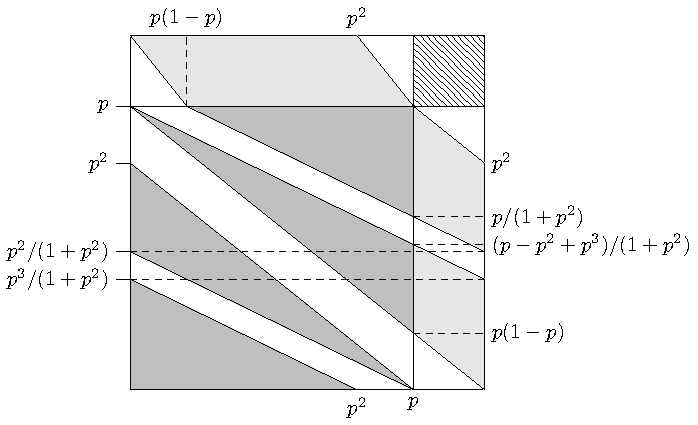
\includegraphics{H-1S}
	\caption{The intersection $H^{-1}(S) \cap S = R_{1,1}$ is shown in dark grey. The pale grey quadrilaterals are the parts of $H^{-1}(S)$ which lie outside $S$, and which will return on a later iterate of $H$. Here we choose $p=0.8$.}
	\label{fig:H-1S}
\end{figure}

A common technique in the study of hyperbolic dynamical systems is to inspect a return map to a hyperbolic set. That is, consider the map $H_S: S \to S$, defined by $H_S = H^k$, where $k$ is such that, for $x \in S$, $H^k(x) \in S$ and $H^j(x) \notin S$ for $j=1, \ldots , k-1$. Such a return map induces a natural partition of $S$ into regions of different return times $k$. This partition is central to the application of Young Tower techniques for computing mixing rates, and $H_S$ was used in \cite{springham2014polynomial} to demonstrate that LTMs have polynomial decay of correlations. Here we observe that $H_S$ partitions $S$ into countably many 
open sets on which $H_S$ is characterised by $DH_S = M_{a,b}$, where $a+b-1 = k$. Typically in decay of correlation arguments only the partition sets for large $k$, and the rate at which they decrease in size, are of interest. Here we construct in detail the entire return time set, and use the notation
$$
R_{a,b} = \{ x | D_x H_S = M_{a,b} \},
$$
that is, $R_{a,b}$ contains those points $x$ for whom $H_S = G_1^b F_1^a$. We characterise the size of the sets $R_{a,b}$ using the conditional measure $\mu_S$, and write
$$
\mu_S(R_{a,b}) = \mu_L(R_{a,b})/p^2,
$$
where $\mu_L$ is Lebesgue measure. Note that $\mu_S$ is an ergodic invariant measure for $H_S$~\cite{przytycki1983ergodicity}. 
% R(a,b) = \mu_S(R_{a,b}) is Birkhoff



%We will now find a return time distribution for points in a specific region of the domain (the region $S$), which will serve as the distribution element of our bounds. Note that throughout this section $F$ and $G$ will refer to the non-identity parts of the maps, $F_1$ and $G_1$. For example, if we say a point $x$ returns to $S$ following application by $GGFF$, we really mean that it returned after application by the sequence $G_1 F_2 G_1 F_1 G_2 F_1$. We also use the following conditional measure for the points in $S$, derived from the Lebesgue measure $\mu_L$:
%\begin{equation}
%\mu_S (A) = \frac{\mu_L (A)}{p^2}.
%\end{equation}
%
%We require a matrix to be hyperbolic in order to obtain its invariant cone. In the case of the map $H$, an orbit yields a hyperbolic matrix provided it undergoes application by both $F$ and $G$, or in other words, provided the orbit is not just a sequence of either $F$s or $G$s. The following lemma guarantees that orbits beginning in $S$ must yield a hyperbolic matrix upon returning to $S$ for the first time, or equivalently, the return map to $S$ is itself hyperbolic.
%
%\begin{lemma}
%	Let $z = (x,y) \in S$. The return map to $S$ of $z$ under $H$, $H_S$, is hyperbolic, and is of the form
%	\begin{equation}
%	H_S \left( \begin{array}{c} x\\ y \end{array} \right)= \left( \begin{array}{cc} 1 & \frac{k}{p} \\ \frac{n-k+1}{p} & 1 + \frac{k(n-k+1)}{p^2} \end{array} \right) \left( \begin{array}{c} x\\ y \end{array} \right),
%	\end{equation}
%	where $n$ is the number of iterates of $H$ required for $z$ to return to $S$, and $1 \le k \le n$. The only possible sequences through which $z$ can return to $S$ under $H$ are those of the form $G^{n-k+1} F^k$.
%\end{lemma}
%
%\begin{proof}
%	We have two possibilities for $H(X)$ after one iterate: $F$ or $GF$. If $H = F$, then after one iterate of $H$ we find ourselves in $A$. We then must undergo application by only $F$s until we re-enter $S$, at which point we undergo application by at least one $G$, since we apply $G$ after $F$ for a full iterate of $H$. If this application of $G$ moves us into $B$, then we udergo application by only $G$s until we next re-enter $S$, at which point we have returned. Hence the sequences $G^{n-k+1} F^k$ are possible for $k/ge 2$, where $n$ is the number of iterates of $H$. If $H = GF$, then we either return immediately, or find ourselves in $B$. While in $B$ we can only undergo application by $G$s until we return to $S$, hence the sequences $G^n F$ are possible. In other words, the only possible sequences for points in $S$ is a string of $F$s followed by a string of $G$s, of the form $G^{n-k+1} F^k$ for $k \ge 1$.
%	
%	Finally,
%	$$ F^k = \left( \begin{array}{cc} 1 & \frac{k}{p} \\ 0 & 1 \end{array} \right) ,$$
%	$$G^{n-k+1} = \left( \begin{array}{cc} 1 & 0 \\ \frac{n-k+1}{p} & 1 \end{array} \right),$$
%	and the composition of these gives us the required result for $R_X$, which has eigenvalues
%	$$\lambda_\pm = \frac{1+\frac{k(n-k+1)}{p^2} \pm \sqrt{(1+\frac{k(n-k+1)}{p^2})^2 - 4}}{2}.$$
%	Since $n \ge k \ge 1$, we have that $\lambda_+ > 1$ and $0 < \lambda_- < 1$, and hence $R_X$ is hyperbolic.
%\end{proof}

%%%%
% FIG 2
%%%%
\begin{figure}
	\centering
	\begin{tikzpicture}[yscale=6,xscale=6]
	\def\p{0.8}
	\def\r{4}
	\def\s{5}
	\draw[pattern=north west lines, pattern color=black] (\p,\p) rectangle (1,1);
	\draw[fill=gray!50!white](1,0) -- (\p+\p-1,\p-\p^2) -- ({(\p^3-\p^2+\p+\p-1)/(1+\p^2)},{(\p^3-\p^2+\p)/(1+\p^2)}) -- ({1/(1+\p^2)},{(\p^3)/(1+\p^2)}) -- cycle;
	\draw[fill=gray!20!white](1,0) -- (\p,\p-\p^2) -- (\p,{(\p-\p^2)/2}) -- cycle;
	\draw[fill=gray!20!white](\p,\p) -- (1,\p^2) -- (1,{(\p+\p^2)/2}) -- cycle;
	\draw[fill=gray!50!white](0,\p^2) -- (0,{(\p+\p^2)/2}) -- (1-\p,\p^2) -- ({1-(\p)/(1+\p^2)},{(\p^2)/(1+\p^2)}) -- ({(\p^3+\p-1)/(1+\p^2)},{(\p)/(1+\p^2)}) -- cycle;
	\draw[fill=gray!50!white]({(\p-\p^2)/2},\p)--({(-\p^3 + \p^2 -\p - \p + 1)/(\p)+1},\p+\p-1)--(\p,{(\p-\p^2+\p^3)/(1+\p^2)})--(\p,{\p/(1+\p^2)})--({(\p-\p^2)},\p)--cycle;
	\draw[fill=gray!50!white](0,{\p^2/(1+\p^2)})--(0,{\p^3/(1+\p^2)})-- (\p^2,0) -- ({(\p^2+\p)/2},0)--({(\p^3 + \p -1)/(\p)},1-\p)--cycle;
	\draw[fill=gray!20!white](\p,\p)--(\p^2,1)--({(\p^2+\p)/2},1)--cycle;
	\draw[fill=gray!20!white](0,1)--({(\p-\p^2)},\p)--({(\p-\p^2)/2},\p)--cycle;
	\draw[fill=gray!20!white](\p,{\p/(1+\p^2)}) -- (1,{\p^2/(1+\p^2)}) -- (1,{\p^3/(1+\p^2)}) -- (\p,{(\p-\p^2+\p^3)/(1+\p^2)})--cycle;
	\draw [fill=gray!50!white] (\p-\p^2,\p)--(\p,{\p/(1+\p^2)})--(\p,\p)-- 
(\p-\p^2,\p);
	\draw [fill=gray!50!white] (0,\p)--(\p,{(\p-\p^2+\p^3)/(1+\p^2)})--(\p,{\p*(1-\p)}) -- (0,\p);
	\draw [fill=gray!50!white] (0,{\p^2/(1+\p^2)})--(0,\p^2)--(\p,0)--(0,{(\p^2/(1+\p^2)});
	\draw [fill=gray!50!white] (\p^2,0)--(0,0)--(0,{\p^3/(1+\p^2)})--(\p^2,0);
	\draw[dotted] (\p,0) --(\p,1);
	\draw[dotted] (0,\p) --(1,\p);
	\node at ({0.15*\p},{0.15*\p}) {$R_{1,1}$};
	\node at ({0.85*\p},{0.85*\p}) {$R_{1,1}$};
	\node at ({0.88*\p},{0.46*\p}) {$R_{1,1}$};
	\node at ({0.12*\p},{0.52*\p}) {$R_{1,1}$};
	\node at (0.76*\p,0.3*\p) {$R_{2,1}$};
	\node at (0.25*\p,0.7*\p) {$R_{2,1}$};
	\node at (0.3*\p,0.29*\p) {$R_{1,2}$};
	\node at (0.7*\p,0.71*\p) {$R_{1,2}$};
	\node at (0.5*\p,0.5*\p) {\small{$R_{2,2}$}};
	\draw ({(\p*\p*\p+\p-1)/\p},1-\p) {circle (0.5pt)};	
	\draw ({(-\p*\p*\p+\p*\p-\p+1)/\p},{2*\p-1}) {circle (0.5pt)};	
	\draw (0,0)--(1,0)--(1,1)--(0,1)--(0,0);
	\end{tikzpicture}
	\caption{The darker grey regions are the points which return to $S$ after one ($R_{1,1}$) and two ($R_{1,2}$ and $R_{2,1}$) iterates of $H$. The lighter grey regions indicate the points yet to return, which are iterated backwards to obtain the later distribution elements. Of these, the quadrilateral will return on the next iterate to the central white quadrilateral ($R_{2,2}$), while the triangular regions form the sets $R_{n,1}$ and 
$R_{1,n}$ for $n \ge 3$. The circles mark points mentioned in the proof of lemma~\ref{lem:Rsets}.}
	\label{fig:R12}
\end{figure}

In practice, to find the return time distribution, we calculate the pre-images of the set $S$ under $H$, and record the sets of points for which these pre-images intersect~$S$. For example, the set $R_{1,1}$ is the set $H^{-1}(S) \cap S$. Figure~\ref{fig:H-1S} shows the geometrical construction of this procedure, with all the coordinates of the intersections needed to calculate the area of this set. Figure~\ref{fig:R12} continues this 
procedure, to produce the regions which return to $S$ under a second application of $H^{-1}$. 
\begin{lemma}\label{lem:Rsets}
Let $p^3 + p - 1 \ge 0$. Then
\begin{align*}
\mu_S (R_{1,1}) &= \frac{2p^3}{1+p^2}, \\
\mu_S (R_{1,2}) = \mu_S(R_{2,1}) & = \frac{-3p^4+2p^3+2p-1}{2p(1+p^2)}, \\
\mu_S(R_{2,2}) &= \frac{(1-p)^2}{1+p^2}.
\end{align*}
\end{lemma}

\begin{proof}
These are all simple calculations based on the constructions shown in figures~\ref{fig:H-1S} and \ref{fig:R12}. We note that we give the condition 
$p^3 + p - 1 \ge 0$  (or $ p \ge 0.682\ldots$) since if this condition is 
not met, then the change in gradient which occurs at the points $(\frac{p^3+p-1}{p},1-p)$ and $(\frac{-p^3 + p^2 - 2p + 1}{p},2p-1)$ (marked with circles in figure \ref{fig:R12}) will instead be contained within the unreturned regions, and will continue into later iterates, making the return 
time distribution more complicated, but not notionally more difficult.
\end{proof}




The set of unreturned points for $n \ge 2$ consists of $R_{2,2}$, plus four triangles, shown in blue in figure~\ref{fig:R12}. Apart from $R_{2,2}$, the itineraries for such unreturned points are of the form $F^n G$ and $FG^n$, for $n \ge 3$. There are countably many such regions $R_{n,1}$ and~$R_{1,n}$ but these are also simply calculated, and are shown in figure~\ref{fig:R}.
\begin{lemma}\label{lem:Rcountable}
Let $n \ge 3$ and as before $p^3 + p - 1 \ge 0$. Then 
\begin{equation*}
\mu_S(R_{n,1}) = \mu_S(R_{1,n}) = \frac{2(1-p)^2}{np(n-1)(n-2)}.
\end{equation*}
\end{lemma}

\begin{proof}
The set $R_{n,1}$ consists of two triangles, one near $(1,0)$ and one near $(0,1)$. The first of these can be expressed as the difference between triangles $T_n$ and $T_{n-1}$, where the corners of $T_n$ have coordinates $(1,0)$, $(p,p(1-p)/n)$, $(p,p(1-p)/(n-1))$. The area of $T_n$ is $p(1-p)^2/2n(n-1)$ and so $\mu_S(R_{n,1})$ is twice $p(1-p)^2/n(n-1)(n-2)$. The set $R_{1,n}$ is similar.
\end{proof}

%%%%
% FIG 3
%%%%
\begin{figure}
	\centering
	\begin{tikzpicture}[yscale=8,xscale=8]
	\def\p{0.8}
	\draw (\p,{\p*(1-\p)}) --(\p,{\p*(1-\p)/2}) -- (\p+\p-1,\p-\p^2) -- ({(\p^3-\p^2+\p+\p-1)/(1+\p^2)},{(\p^3-\p^2+\p)/(1+\p^2)}) -- ({1/(1+\p^2)},{(\p^3)/(1+\p^2)}) -- cycle;
	\draw(0,\p^2) -- (0,{(\p+\p^2)/2}) -- (1-\p,\p^2) -- ({1-(\p)/(1+\p^2)},{(\p^2)/(1+\p^2)}) -- ({(\p^3+\p-1)/(1+\p^2)},{(\p)/(1+\p^2)}) -- cycle;
	\draw({(\p-\p^2)/2},\p)--({(-\p^3 + \p^2 -\p - \p + 1)/(\p)+1},\p+\p-1)--(\p,{(\p-\p^2+\p^3)/(1+\p^2)})--(\p,{\p/(1+\p^2)})--({(\p-\p^2)},\p)--cycle;
	\draw(0,{\p^2/(1+\p^2)})--(0,{\p^3/(1+\p^2)})-- (\p^2,0) -- ({(\p^2+\p)/2},0)--({(\p^3 + \p -1)/(\p)},1-\p)--cycle;
	\draw  (\p-\p^2,\p)--(\p,{\p/(1+\p^2)})--(\p,\p)-- (\p-\p^2,\p);
	\draw (0,\p)--(\p,{(\p-\p^2+\p^3)/(1+\p^2)})--(\p,{\p*(1-\p)}) -- (0,\p);
	\draw (0,\p^2)--(\p,0);
	\draw (\p,0)--(0,{(\p^2/(1+\p^2)});
	\draw (\p^2,0)--(0,0)--(0,{\p^3/(1+\p^2)})--(\p^2,0);

	\foreach \j in {1,...,20}{
		\draw (\p,{\p*(1-\p)/(\j+1)})--({((\j+1)*\p-1)/\j},{\p*(1-\p)/\j});
		\draw (0,{\p-\p*(1-\p)/(\j+1)})--({\p-((\j+1)*\p-1)/\j},{\p-\p*(1-\p)/\j});
		\draw ({\p*(1-\p)/(\j+2)},\p)  -- ({(\p*\p-\p*\p*\p+1-\p)/((\j+1)*\p)},{((\j+2)*\p-1))/(\j+1)});
		\draw ({\p-\p*(1-\p)/(\j+2)},0)  -- ({\p-((\p*\p-\p*\p*\p+1-\p)/((\j+1)*\p))},{\p-(((\j+2)*\p-1))/(\j+1))});
}

	\node at ({0.15*\p},{0.15*\p}) {\small{$R_{1,1}$}};
	\node at ({0.85*\p},{0.85*\p}) {\small{$R_{1,1}$}};
	\node at ({0.88*\p},{0.46*\p}) {\small{$R_{1,1}$}};
	\node at ({0.12*\p},{0.52*\p}) {\small{$R_{1,1}$}};
	\node at (0.76*\p,0.3*\p) {\small{$R_{2,1}$}};
	\node at (0.25*\p,0.7*\p) {\small{$R_{2,1}$}};
	\node at (0.3*\p,0.29*\p) {\small{$R_{1,2}$}};
	\node at (0.7*\p,0.71*\p) {\small{$R_{1,2}$}};
	\node at (0.5*\p,0.5*\p) {\scriptsize{$R_{2,2}$}};

	\node at (\p,0.02)[right] {\small{$R_{n,1}$}};
	\node at (\p-0.02,0.0)[below] {\small{$R_{1,n}$}};	
	\node at (0,\p-0.02)[left] {\small{$R_{n,1}$}};
	\node at (0.02,\p)[above] {\small{$R_{1,n}$}};	
	

	\draw (0,0)--(\p,0)--(\p,\p)--(0,\p)--(0,0);
	\end{tikzpicture}
	\caption{The complete return time partition, shown here for $p=0.8$.  }
	\label{fig:R}
\end{figure}



To complete the proof of theorem \ref{thm:simple_bounds} we recognise that the required frequency with which $M_{a,b}$ appears along an orbit of $H$ is exactly the relative size of the subset of~$S$ for which the return 
map $H_S$ is equal to $G_1^b F_1^a$. That is, $R(a,b) = \mu_S(R_{a,b})$. This is an immediate consequence of theorem \ref{thm:birkhoff} with $\phi =  \chi_{R_{a,b}}$. Finally, we require $n_S$. This 
can be computed directly from the expectation 
\begin{align*}
n_S &= \langle a+b-1 \rangle =\sum_{a,b} (a+b-1) R(a,b) \\
& = R(1,1) + 2(R(1,2)+R(2,1)) +3R(2,2) + \sum_{n = 3}^\infty n (R(1,n) + R(n,1))\\
& = \frac{-4p^4+7p^3-6p^2+7p-2}{p(1+p^2)} + \frac{4(1-p)^2}{p} \sum_{n = 3}^\infty \frac{1}{(n-1)(n-2)}\\
& = \frac{-4p^4+7p^3-6p^2+7p-2}{p(1+p^2)} + \frac{4(1-p)^2}{p} \sum_{m = 1}^\infty \frac{1}{m(m+1)}\\
& = \frac{-4p^4+7p^3-6p^2+7p-2}{p(1+p^2)} + \frac{4(1-p)^2}{p}\\
& = \frac{2}{p} - 1.
\end{align*}
Alternatively, we can apply Kac's lemma \cite{kac1947notion},  which states that for an ergodic, measure-preserving transformation, the expected first return time to a set $S$ is $1/ \mu(S)$, where $\mu$ is the normalized measure on the domain. Since $\mu(S) = p^2$ and $\mu(P \cap Q) = 1-(1-p)^2 = p(2-p)$ we have $n_S = p(2-p)/p^2 = 2/p-1$, confirming the validity of the return time distribution in this section.





\section{Improving the bounds}\label{sec:improve}

Here we discuss the circumstances under which we can consider narrower cones than~$C$, in order to improve upon the bounds 
$\Psi_{H,k}$ and $\Phi_{H,k}$ in Theorem \ref{thm:simple_bounds}. In \cite{sturman2019lyapunov}, the case of bounding random products of matrices, the corresponding modifications were relatively simple, as the frequency with which the matrix $M_{a_2,b_2}$ preceded the matrix~$M_{a_1,b_1}$ in any orbit was independent of the choice of $a_1$ and $b_1$. In the present deterministic case, however, this independence does not hold. 

Instead, we consider which matrices $M_{a_2,b_2}$ can precede each $M_{a_1,b_1}$. The benefit of doing so is to replace the cone $C$ with its narrower image $M_{a_2,b_2} (C)$, improving the bounds of lemma \ref{lem:Mabbounds}. 


\begin{figure}
	\centering
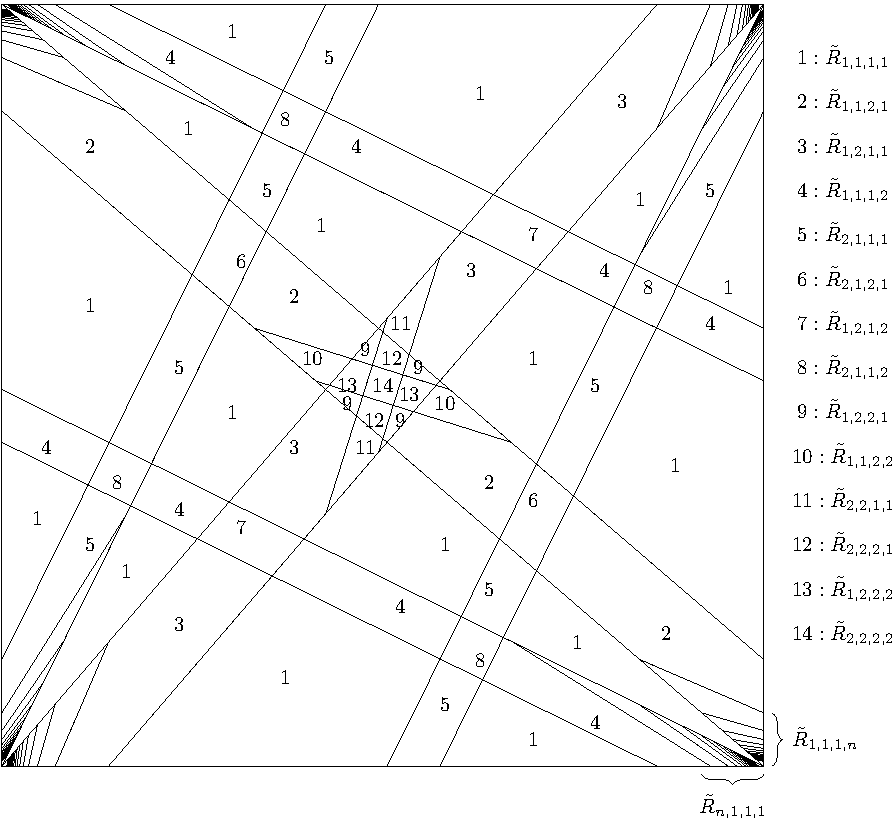
\includegraphics[width=0.75\linewidth]{double_partition_fig.pdf}
\caption{The partition depicting $\{ x | H_S^2 = F_1^{a_2} G_1^{b_2} F_1^{a_1} G_1^{b_1}\}$ for $a_1, a_2, b_1, b_2 \in \{ 1, 2, 3 \ldots \}$.}\label{fig:improved_partition}
\end{figure}

\begin{lemma}\label{lem:better_Mabbounds}
We have
$$
\tilde{\psi}_k (a_2,b_2,a_1,b_1) \le \frac{\| M_{a_1,b_1} v  \|_k}{\| v  \|_k} \le \tilde{\phi}_k (a_2,b_2,a_1,b_1)
$$
for $k \in \{ 1,2,\infty \}$ and $v \in M_{a_2,b_2} (C)$, with
\begin{align*}
\tilde{\psi}_{\infty} &= 1+\frac{a_1 b_1}{p^2} + \frac{a_2 b_1}{p^2 + a_2b_2}\\
\tilde{\phi}_{\infty} &= 1+\frac{a_1 b_1}{p^2} + \frac{b_1 p^2+a_2 b_1}{p^2(1+b_2) + a_2 b_2}\\
\tilde{\psi}_{1} &= 1+\frac{a_1p^3+(a_2b_1+a_1b_1)p^2+a_2a_1b_2p+a_1a_2b_1b_2}{p^2(a_2b_2+a_2p+p^2)}\\
\tilde{\phi}_{1} &= 1+\frac{b_1p^4+(a_1b_2+a_1)p^3+(b_2a_1b_1+a_2b_1+a_1b_1)p^2+a_1a_2b_2p+a_1a_2b_1b_2}{p^2(p^3+(b_2+1)p^2+a_2p+a_2b_2)} \\
\tilde{\psi}_2 &= \min \{ \xi_1,\xi_2  \}   \\
\tilde{\phi}_2 &=   \begin{cases} \sqrt{\lambda_{M_{a_1,b_1}^T M_{a_1,b_1}}^{u}}  & \mbox{if  $ v_{max}^2 \in M_{a_2,b_2} (C)$} \\
\max \{ \xi_1,\xi_2 \}  & \mbox{otherwise},
\end{cases}
\end{align*}
where
\begin{align*}
\xi_1 &=   \frac{\sqrt{\left(\frac{a_{1} \left(a_{2} b_{2} + p^2\right)}{p^3} + \frac{a_{2}}{p}\right)^{2} + \left(\frac{a_{2} b_{1}}{p^{2}} + \left(\frac{a_{1} b_{1}}{p^{2}} + 1\right) \left(\frac{a_{2} b_{2}}{p^{2}} + 1\right)\right)^{2}}}{\sqrt{\frac{a_{2}^{2}}{p^{2}} + \left(\frac{a_{2} b_{2}}{p^{2}} + 1\right)^{2}}} \\
\xi_2 &= \frac{\sqrt{\left(\frac{b_{1} \left(a_{2} + p^2\right)}{p^2} + \left(\frac{a_{1} b_{1}}{p^{2}} + 1\right) \left(\frac{a_{2} b_{2}}{p^{2}} + b_{2} + 1\right)\right)^{2} + \left(\frac{a_{1} \left(a_{2} b_{2} + p^2(b_{2} + 1)\right)}{p^3} + \frac{a_{2}}{p} + p\right)^{2}}}{\sqrt{\left(\frac{a_{2}}{p} + p\right)^{2} + \left(\frac{a_{2} b_{2}}{p^{2}} + b_{2} + 1\right)^{2}}}
\end{align*}
\end{lemma}

\begin{proof}
Similarly to lemma~\ref{lem:Mabbounds}, $\| M_{a_1,b_1} v  \|_k/\| v  \|_k$ changes monotonically in $M_{a_2,b_2} (C)$ in the $l_1$ and $l_{\infty}$ cases. In the $l_2$ case, the maximising vector $ v_{max}^2 $ may or may not be contained in the cone $M_{a_2,b_2} (C)$. The calculations are again elementary. 
\end{proof}

To complete the improved bounds, we require the proportion of a typical orbit which sees $M_{a_2,b_2}$ followed by $M_{a_1,b_1}$. To obtain this we calculate the measure of the set of points in $R_{a_2,b_2}$ which map under the return map $H_S$ into $R_{a_1,b_1}$, that is, $\mu ( \{ x | H_S^2 = F_1^{a_2}G_1^{b_2}F_1^{a_1}G_1^{b_1} \} )$. Since $H$ is $\mu$-invariant we have
$$
\mu (R_{a_2,b_2} \cap H_S^{-1} (R_{a_1,b_1})) = \mu (H_S(R_{a_2,b_2}) \cap  R_{a_1,b_1}) 
$$
and we use the notation $H_S(R_{a_2,b_2}) \cap  R_{a_1,b_1} = \tilde{R}_{a_2,b_2,a_1,b_1} $. So we consider the partition in figure~\ref{fig:R} and its forward image, which by the symmetry of the map is simply the original partition rotated through $90^{\circ}$. The partition and its image 
is shown in figure~\ref{fig:improved_partition}. The size of each region of this `improved partition' can be calculated using simple geometry. The 
task is made simpler by the fact that the countably infinite regions of the original partition do not intersect with their own images, that is, for $n\ge 3$,
$$
H_S(R_{1,n} \cup R_{n,1} ) \cap (R_{1,n} \cup R_{n,1}) = \emptyset
$$
(noted as Lemma 3.2 of \cite{springham2014polynomial}) and moreover the symmetry induces the relationship
$$
\mu_S (\tilde{R}_{a_2,b_2,a_1,b_1}) = \mu_S (\tilde{R}_{b_1,a_1,b_2,a_2})
$$
for all $a_1, b_1, a_2, b_2$. The areas $\mu_S(\tilde{R}_{a_2,b_2,a_1,b_1})$ are given in:
\begin{lemma}\label{lem:R_HR}
\begin{align*}
\mu_S(\tilde{R}_{1,1,1,1}) &= \frac{p \left(12 p^{8} + 28 p^{6} - 12 p^{5} + 14 p^{4} - 16 p^{3} + 6 p^{2} - 4 p + 2\right)}{2 p^{8} + 9 p^{6} + 
12 p^{4} + 6 p^{2} + 1} \\
\mu_S(\tilde{R}_{1,1,1,2}) &= \mu(\tilde{R}_{2,1,1,1}) \\
&\hspace{-8ex} = - \frac{\left(10 p^{10} + 4 p^{9} + 9 p^{8} - 10 p^{7} 
+ p^{6} - 24 p^{5} + 14 p^{4} - 12 p^{3} + 9 p^{2} - 2 p + 1\right)}{4 p^{9} + 18 p^{7} + 24 p^{5} + 12 p^{3} + 2p}   \\
\mu_S(\tilde{R}_{1,1,2,1}) &=\mu(\tilde{R}_{1,2,1,1}) =   - \frac{8 p^{6} - 4 p^{5} - 6 p^{3} + p^{2} + 1}{4 p^{5} + 6 p^{3} + 2p} \\
\mu_S(\tilde{R}_{1,1,2,2}) &=\mu(\tilde{R}_{2,2,1,1}) =  \frac{ \left(- p^{3} + 4 p^{2} - 5 p + 2\right)}{2 \left(p^{2} + 1\right)}  \\
\mu_S(\tilde{R}_{1,2,1,2}) &=\mu(\tilde{R}_{2,1,2,1}) =  \frac{2 p \left(p^{2} - 2 p + 1\right)}{2 p^{2} + 1}  \\
\mu_S(\tilde{R}_{1,2,2,1}) &=  \frac{ \left(- p^{5} + 4 p^{4} - 9 p^{3} 
+ 14 p^{2} - 12 p + 4\right)}{p^{4} + 5 p^{2} + 4}  \\
\mu_S(\tilde{R}_{1,2,2,2}) &= \mu(\tilde{R}_{2,2,2,1}) = \frac{p \left(p^{4} - 4 p^{3} + 9 p^{2} - 10 p + 4\right)}{2 \left(p^{4} + 5 p^{2} + 4\right)}   \\
\mu_S(\tilde{R}_{2,1,1,2}) &= \frac{4 p^{2} \left(p^{2} - 2 p + 1\right)}{p^{4} + 3 p^{2} + 1}   \\
\mu_S(\tilde{R}_{2,2,2,2}) &=   \frac{p^{2} \left(p^{2} - 2 p + 1\right)}{p^{4} + 5 p^{2} + 4}  \\
\mu_S(\tilde{R}_{n,1,1,1}) &= \mu_S(\tilde{R}_{1,n,1,1}) = \mu_S(\tilde{R}_{1,1,n,1}) = \mu_S(\tilde{R}_{1,1,1,n}) = \frac{2(1-p)^2}{np(n-1)(n-2)}.
\end{align*}
In each case, by theorem~\ref{thm:birkhoff}, we have $\tilde{R}(a_2,b_2,a_1,b_1) = \mu_S( \tilde{R}_{a_2,b_2,a_1,b_1})$. 
\end{lemma}

\begin{proof}
The computation of these areas are all the result of simple geometry, illustrated in figure~\ref{fig:improved_partition}. 
\end{proof}

Replacing the functions $\phi_k$, $\psi_k$ and $R$ of theorem \ref{thm:simple_bounds} with $\tilde{\phi}_k$, $\tilde{\phi}_k$ and $\tilde{R}$ completes the proof of theorem~\ref{thm:better_bounds}.


\section{Discussion}\label{sec:discuss}

\subsection{Accuracy of the bounds}

The bounds on $\lambda$ given by theorems \ref{thm:simple_bounds} and \ref{thm:better_bounds} can be computed easily and rapidly. Here we compare the numerical values of these bounds with values produced by a standard numerical algorithm \cite{parker2012practical} using Gram-Schmidt orthonormalisation to quantify the exponential growth of tangent vectors implicit 
in a positive Lyapunov exponent. The bounds $\Phi_{H,k}$ and $\Psi_{H,k}$ each involve an infinite sum, but truncating these at some large but finite limit give accurate evaluations. In particular, since every term in each sum is positive, any truncation of $\Psi_{H,k}$ is a strict lower bound, while each term decreases roughly as $n^{-3}\log n$. 
\begin{figure}
     \centering
     \begin{subfigure}[b]{0.49\textwidth}
         \centering
         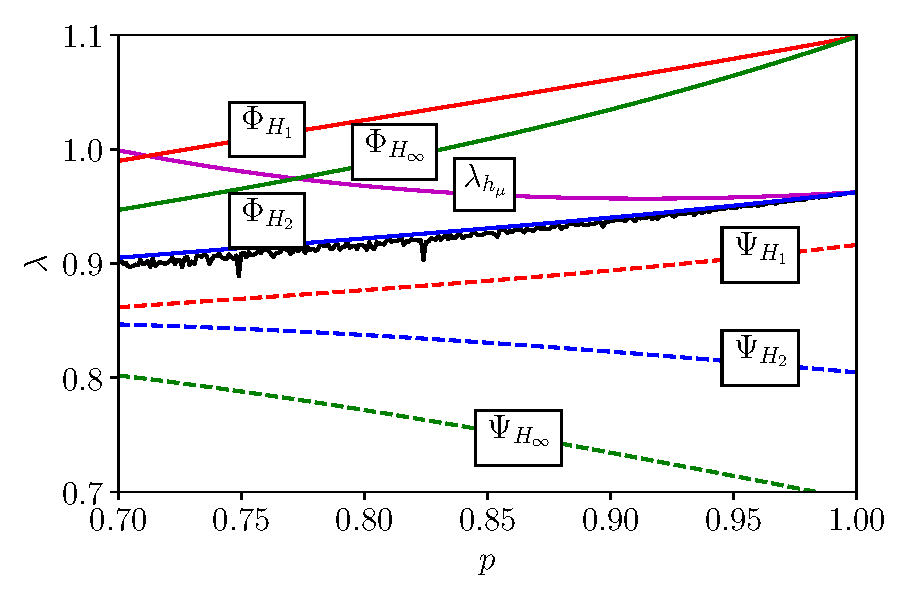
\includegraphics[width=\textwidth]{ltm_simple_bounds_bw.pdf}
         \caption{All upper and lower bounds from theorem \ref{thm:simple_bounds}.}
         \label{fig:simple_bounds}
     \end{subfigure}
     \hfill
     \begin{subfigure}[b]{0.49\textwidth}
         \centering
         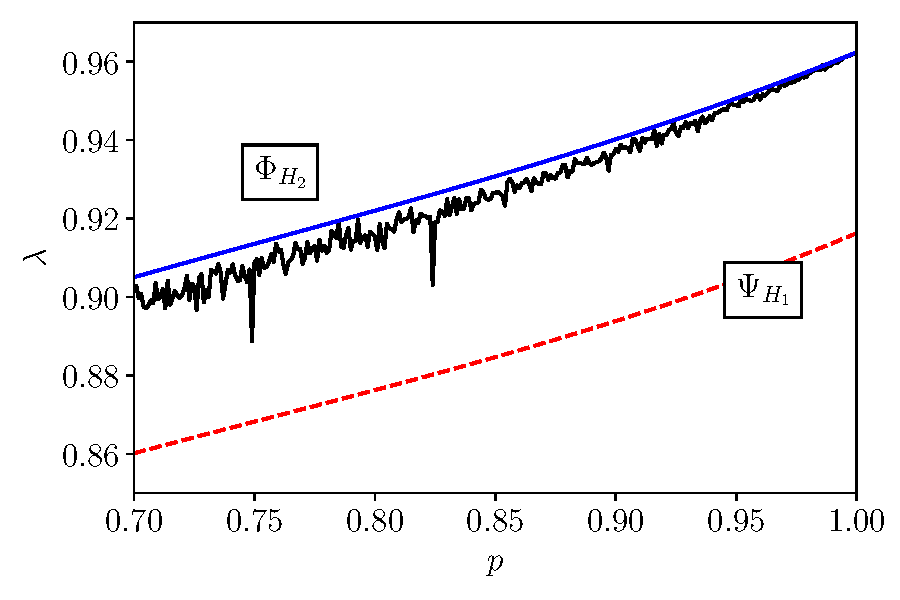
\includegraphics[width=\textwidth]{ltm_simple_bounds_zoom.pdf}
         \caption{Sharpest bounds result from using $l_2$ for the upper bound, and $l_1$ for the lower. }
         \label{fig:simple_bounds_zoom}
     \end{subfigure}
        \caption{(Colour online). Bounds of $\lambda$ given by theorem \ref{thm:simple_bounds}. The black line shows the numerically computed value of $\lambda$. Upper bounds are shown as solid lines, lower bounds as dashed lines. As labelled, and in later figures, red lines originate from the $l_1$ norm, blue lines from the $l_2$ norm, and green lines from the $l_{\infty}$ norm. The magenta line indicates the upper bound from maximising $\lambda_{h_{\mu}}$.} 
        \label{fig:simple}
\end{figure}

Figure~\ref{fig:simple} shows the bounds $\Phi_{H,k}$ and 
$\Psi_{H,k}$ for each of the $L_1$ (red), $L_2$ (blue), $L_{\inf}$ (green) norms. The numerically calculated value for $\lambda$, from $10^6$ iterates of the standard orthonormalisation scheme, is shown as a solid black line. Upper bounds are shown as solid lines, and lower as dashed lines. 
Figure~\ref{fig:simple_bounds} shows that the tightest upper bound comes from the $L_2$ norm, while the tightest lower bound comes from the $L_1$ norm. The bound given by the topological entropy calculation of \cite{DAlessandro1999} is shown in magenta. Note that the upper bound $\Phi_{H,2}$ coincides with $\lambda$ at $p=1$. This is because the vector $v^2_{max} \in C$ given in the proof of lemma~\ref{lem:Mabbounds} is equal to the expanding eigenvector of $H$ when $p=1$. The upper bounds for $L_1$ and $L_{\infty}$ also coincide at $p=1$, where the expressions in lemma~\ref{lem:Mabbounds} are equivalent. Figure~\ref{fig:simple_bounds_zoom} selects the best bounds, and shows that $\Phi_{H,2}$ is considerably tighter than $\Psi_{H,1}$, but still appears greater than the numerically calculated value for all $p<1$. 


\begin{figure}
     \centering
     \begin{subfigure}[b]{0.49\textwidth}
         \centering
         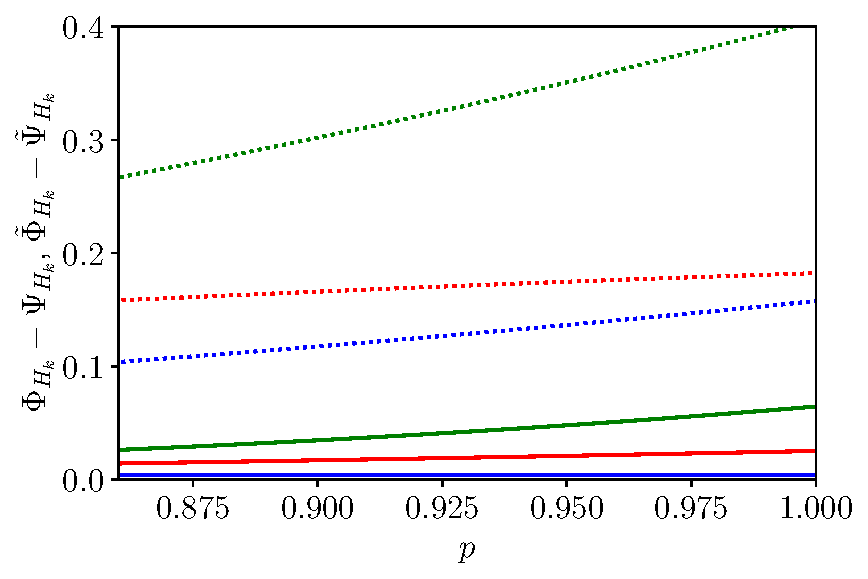
\includegraphics[width=\textwidth]{ltm_better_bounds.pdf}
         \caption{Distance between upper and lower bounds from theorem \ref{thm:simple_bounds} shown dotted, and from theorem \ref{thm:better_bounds} as solid lines.}
         \label{fig:better_bounds}
     \end{subfigure}
     \hfill
     \begin{subfigure}[b]{0.49\textwidth}
         \centering
         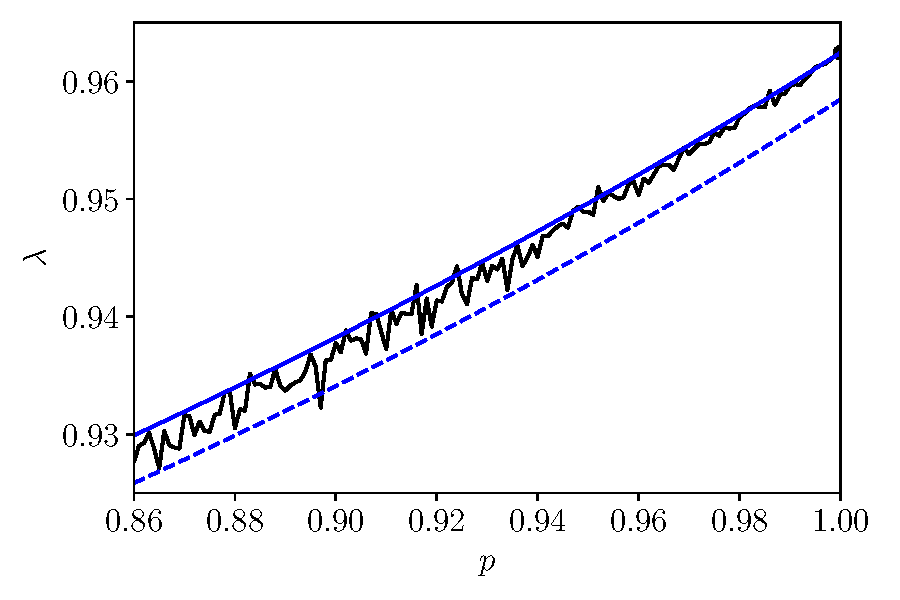
\includegraphics[width=\textwidth]{ltm_better_bounds_zoom.pdf}
         \caption{The sharpest bounds, using the $l_2$ norm, improve on the numerical calculation of $10^6$ iterates.}
         \label{fig:better_bounds_zoom}
     \end{subfigure}
        \caption{(Colour online). Bounds of $\lambda$ given by theorem \ref{thm:better_bounds}. The black line shows the numerically computed value of $\lambda$.}
        \label{fig:better}
\end{figure}
Figure~\ref{fig:better} shows the bounds $\tilde{\Phi}_{H,k}$ and $\tilde{\Psi}_{H,k}$. Here we plot $\Phi_{H,k}-\Psi_{H,k}$ and $\tilde{\Phi}_{H,k}-\tilde{\Psi}_{H,k}$ (in figure~\ref{fig:better_bounds}) to show the improvement in using the return partition 
and its image. Figure~\ref{fig:better_bounds_zoom} shows the bounds using 
the $L_2$ norm, the tightest bounds, and illustrates that the envelope $\tilde{\Phi}_{H,2}-\tilde{\Psi}_{H,2}$ is often narrower than the uncertainty in the numerically calculated value of $\lambda$, even after $10^6$ iterates.

%\jitse{For theorem 2, the $L_1$ norm gives the best lower bound. The last sentence implies that for theorem 3, the $L_2$ norm gives the best lower bound. Is that true? If so, we might want to say that explicitly.}




\subsection{Related quantities}

The method described here could also be used to bound related quantities. 
For example, of interest in many applications is the {\em generalized Lyapunov exponent} $\ell(q)$, which gives the growth rate of the $q$-th moment of a matrix product norm~\cite{crisanti_generalized_1988}. The generalized Lyapunov exponent is used in large deviation theory, and is typically defined for products of random matrices. In this deterministic setting we have
\begin{equation}\label{eq:gle}
\ell(q) = \lim_{n \to \infty} \frac{1}{n} \log \langle \|D_x f^n v_0 \|^q \rangle
\end{equation}
where the average is taken over the invariant measure $\mu$. This is related to the standard Lyapunov exponent by $\lambda = \ell'(0)$. This quantity is notoriously difficult to compute numerically~\cite{vanneste2010estimating}, because fluctuations along a finite orbit are magnified for large 
$q$. However, the expressions in theorems~\ref{thm:simple_bounds} and \ref{thm:better_bounds} can be easily adapted to give quick and accurate upper and lower bounds for $\ell(q)$, since the contributions from averaging 
over the invariant measure are given explicitly by $R(a,b)$. These bounds 
are shown, for the $l_2$ norm, in figure \ref{fig:ltm_gle}. Note that $\ell(q)$ is monotonic, since the existence of the invariant cone means that 
a vector is expanded by DH at every iterate of the map. Generalized Lyapunov exponents are closely related to the joint spectral radius, a quantity which can also be rigorously bounded, for each $l_p$ norm, by this method. 

\begin{figure}
\centering
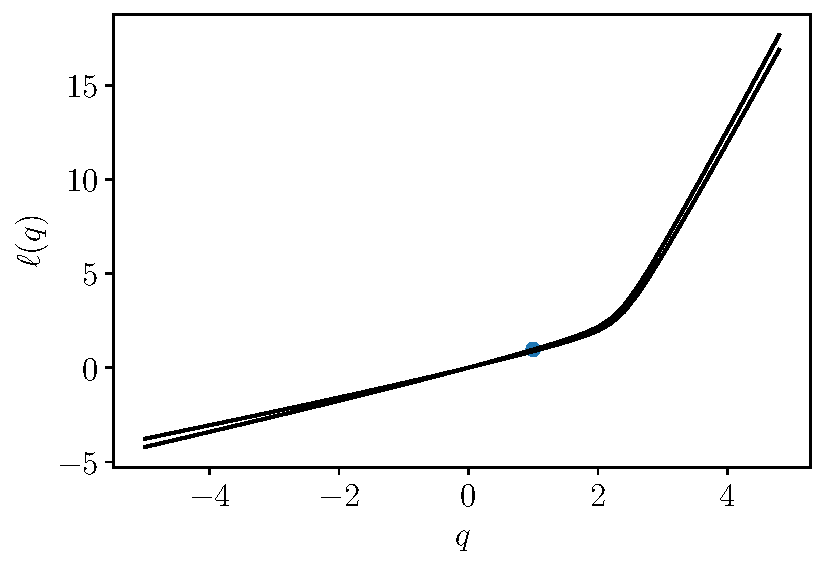
\includegraphics[width=0.75\linewidth]{ltm_gle.pdf}
\caption{Rigorous upper and lower bounds on the generalized Lyapunov exponent $\ell(q)$ for the linked twist map $H$, defined by equation (\ref{eq:gle}), using the $l_2$ norm. The circle indicates $\ell(1)$, which corresponds to the topological entropy $\lambda_{h_\mu} =  \log(1+1/2p^2 + \sqrt{1/p^2+1/4p^2})$.}\label{fig:ltm_gle}
\end{figure}

\subsection{Convergence of Lyapunov exponents}

Finally, we comment on the difficulty of computing Lyapunov exponents numerically for linked twist maps. The standard algorithm \cite{parker2012practical} is not difficult to code, and as the system is low-dimensional and discrete time, is quick to run. However, as shown in figure \ref{fig:better_bounds_zoom}, a large number of iterates is required to improve on the rigorous bounds  presented. Indeed the numerical calculation shows poor convergence to the expected values of $\lambda$, which should change smoothly with $p$. Typically, Lyapunov exponents converge according to the 
central limit theorem. Linked twist maps, however, have slow correlation decay (shown in \cite{springham2014polynomial} to be polynomial, with rate $1/n$). This results in a central limit theorem with a non-standard scaling factor of $\sqrt{n \log n}$, and so slower convergence than usual \cite{mohr2013martingale}.	

\section*{References}
\bibliography{hypshears}

\end{document}